\frame{
  \frametitle{AVL Trees\footnote{Adelson-Velsky, Georgy; Landis, Evgenii (1962)}}
  
  \begin{columns}
    \begin{column}{0.4\textwidth}
    \begin{itemize}
    \item First $O(\log n)$ self-balancing binary search tree!
    
    \medskip
    
    \item Ensures the height of its children do not differ by $>1$
  \end{itemize}
  
  \bigskip
  
  {\tiny \texttt{https://commons.wikimedia.org/w/index.php?curid=49182185}}
    \end{column}
    \begin{column}{0.6\textwidth}  %%<--- here
        \begin{center}
  \includesvg[scale=0.3]{slides/alphabet_trees/AVL-tree-wBalance_K.svg}
  \end{center}
    \end{column}
    \end{columns}
}

\frame{
  \frametitle{AVL Trees (Rotation)}
  \begin{columns}
      \begin{column}{0.35\textwidth}
      \begin{itemize}
          \item Imbalances are fixed by rotations, fundamental local operations for many balanced BSTs
      \end{itemize}
      \end{column}
      \begin{column}{0.65\textwidth}
          \begin{center}
          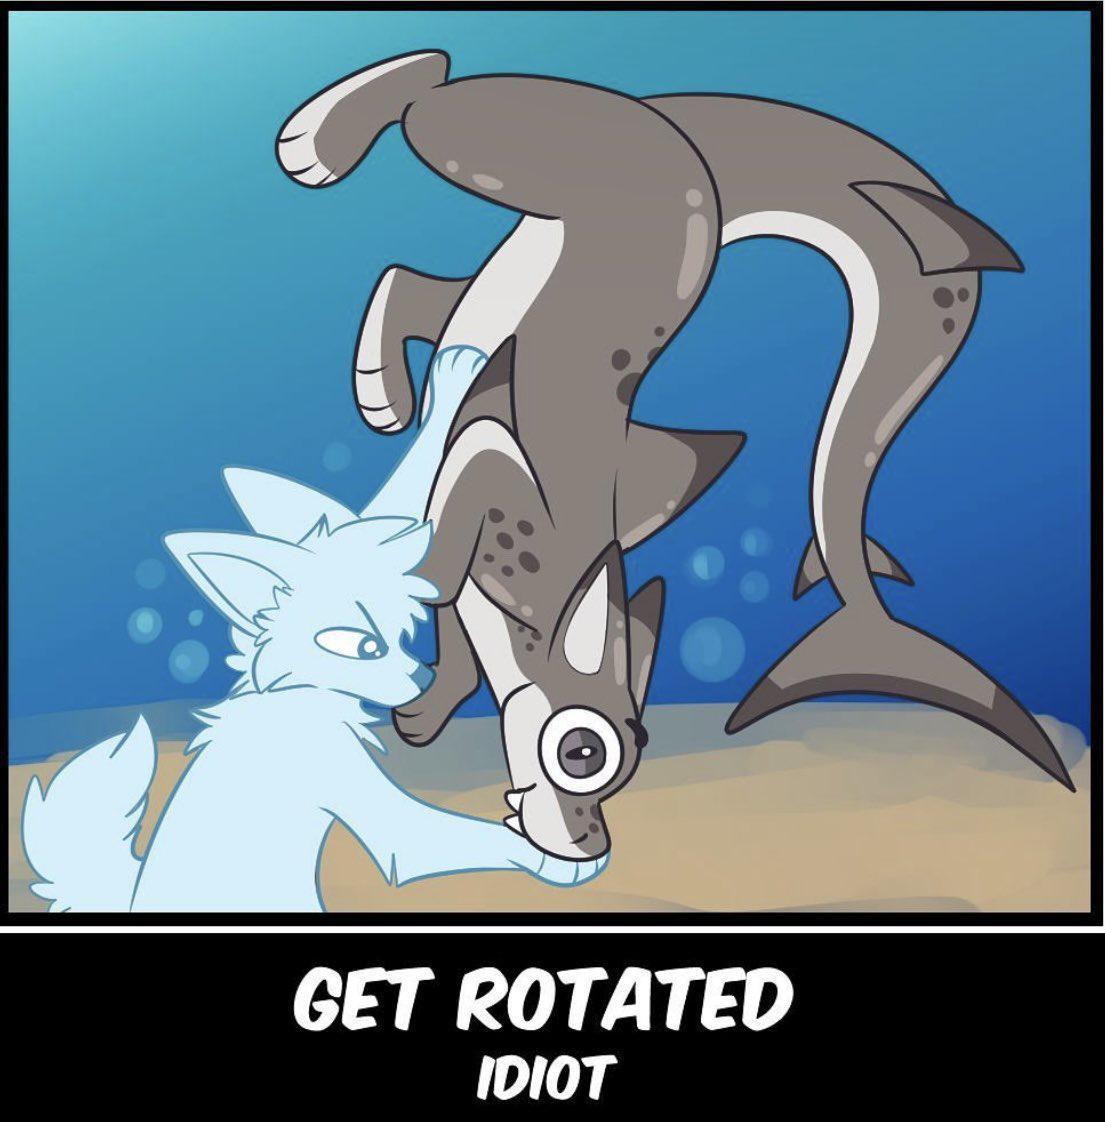
\includegraphics[scale=0.13]{slides/alphabet_trees/furry_getrotated.jpeg}
          
            {\tiny \texttt{/r/furry\_irl/comments/1dumfg3/}}
          \end{center}
      \end{column}
  \end{columns}
  

}

\frame{
  \frametitle{AVL Trees (Rotation)}
  \begin{columns}
      \begin{column}{0.35\textwidth}
      \begin{itemize}
          \item Imbalances are fixed by rotations, fundamental local operations for many balanced BSTs
      \end{itemize}
      \end{column}
      \begin{column}{0.65\textwidth}
          \begin{center}
    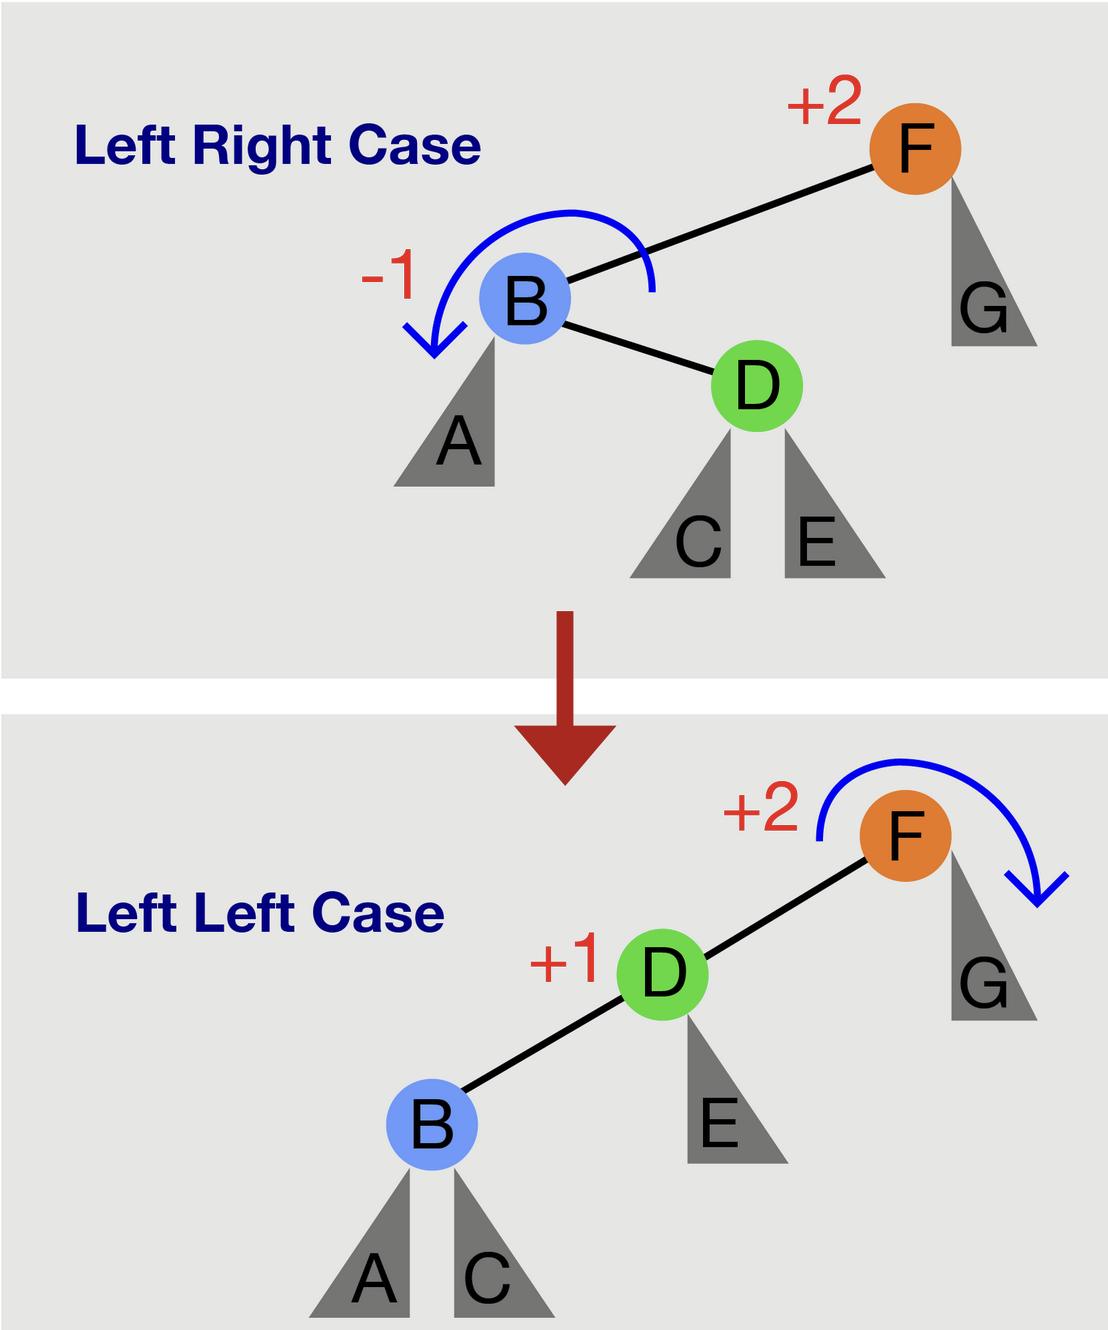
\includegraphics[scale=0.12]{slides/alphabet_trees/bst_rotate.png}
    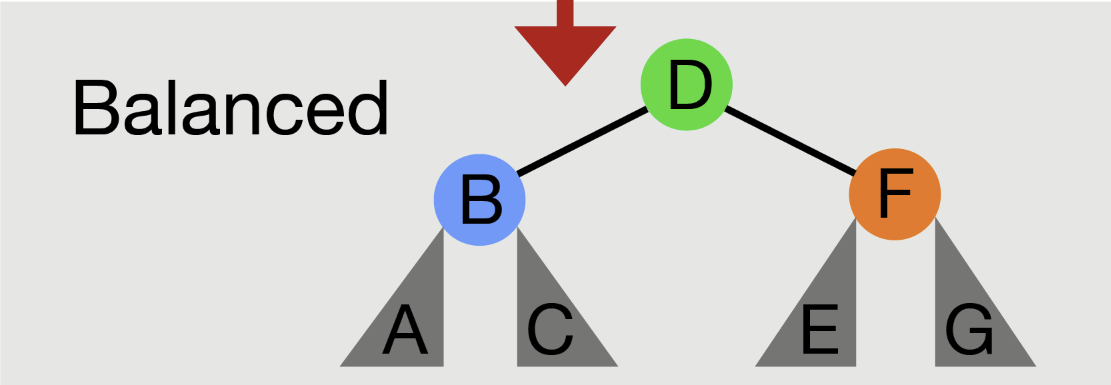
\includegraphics[scale=0.12]{slides/alphabet_trees/bst_balanced.png}
    
    {\tiny \texttt{https://pages.cs.wisc.edu/\texttildecenter qingyi/}}
  \end{center}
      \end{column}
  \end{columns}
  

}